\setcounter{ex}{0} %Thái Hòa-Nghệ An
\subsection{Trắc nghiệm (2 điểm)}
\Opensolutionfile{ans}[ans/ans8]

%%Câu 1:
\begin{ex}
Hai đường thẳng $x+by=6$, $ax+by=12$ cùng đi qua điểm $(3;-3)$. Giá trị của $a$ và $b$ là
\choice
{\True $a=3;b=-1$}
{$a=4;b=-1$}
{$a=4;b=0$}
{$a=3;b=0$}
\end{ex}

%%Câu 2:
\begin{ex}
Giá trị của biểu thức $P=\dfrac{1}{\sqrt{7}-\sqrt{5}}-\dfrac{1}{\sqrt{7}+\sqrt{5}}$ bằng
\choice
{$\sqrt{7}$}
{\True $\sqrt{5}$}
{$2\sqrt{5}$}
{$\sqrt{35}$}
\end{ex}

%%Câu 3:
\begin{ex}
Tính giá trị biểu thức
$F=12\tan32^\circ\tan58^\circ+\sin^251^\circ+\sin^239^\circ-\dfrac{8\cot35^\circ}{\tan55^\circ}$.
\vspace{0.35cm}
\choice
{$3$}
{\True $5$}
{$4$}
{$2$}
\end{ex}

%%Câu 4:
\begin{ex}
Cho hai đường tròn $(O;8\,\text{cm})$ và $(O';3\,\text{cm})$ có $OO'=10\,\text{cm}$. Khẳng định nào sau đây đúng?
\choice
{Hai đường tròn ở ngoài nhau}
{Hai đường tròn tiếp xúc trong}
{\True Hai đường tròn cắt nhau tại hai điểm}
{Hai đường tròn tiếp xúc ngoài}
\end{ex}

%%Câu 5:
\begin{ex}
Cho tam giác $ABC$ vuông tại $A$, đường cao $AH$ có $AB=13\,\text{cm}$; $BH=1{,}1\,\text{dm}$. Tính tỉ số lượng giác $\sin C$ (làm tròn đến chữ số thập phân thứ $2$).
\choice
{$0{,}65$}
{\True $0{,}85$}
{$0{,}95$}
{$0{,}75$}
\end{ex}

%%Câu 6:
\begin{ex}
Một khu du lịch bán hai loại vé tham quan: vé người lớn giá $80\,000$ đồng và vé trẻ em giá $50\,000$ đồng. Trong một buổi sáng, khu du lịch bán được $15$ vé và thu về tổng cộng $960\,000$ đồng. Hỏi khu du lịch đã bán được bao nhiêu vé người lớn?
\choice
{$6$ vé}
{\True $7$ vé}
{$8$ vé}
{$9$ vé}
\end{ex}

%%Câu 7:
\begin{ex}
Điều kiện xác định của căn thức $\sqrt{x+2}$ là
\choice
{$x\le -2$}
{$x\ne -2$}
{\True $x\ge -2$}
{$x>-2$}
\end{ex}

%%Câu 8:
\begin{ex}
Tìm tất cả các giá trị của tham số $m$ để bất phương trình $(m-2)x>m-2$ có tập nghiệm là $x<1$.
\choice
{$m>2$}
{$m=2$}
{\True $m<2$}
{$m\le 2$}
\end{ex}

%%Câu 9:
\begin{ex}
Cho hình quạt tròn có bán kính $6\,\text{cm}$ và độ dài cung tròn tương ứng là $4\pi\,\text{cm}$. Diện tích hình quạt tròn đó bằng
\choice
{$8\pi\,\text{cm}^2$}
{$10\pi\,\text{cm}^2$}
{$16\pi\,\text{cm}^2$}
{\True $12\pi\,\text{cm}^2$}
\end{ex}

%%Câu 10:
\begin{ex}
Cho phương trình $(2m-1)x=m+3$ với $m$ là tham số. Tìm giá trị của $m$ để phương trình vô nghiệm.
\choice
{$m=-3$}
{$m=0$}
{\True $m=\dfrac{1}{2}$}
{$m=3$}
\end{ex}


\Closesolutionfile{ans}
\Opensolutionfile{ansbook}[ans/ansbook8]
\setcounter{bt}{0}
\subsection{Tự luận (8 điểm)}

%Bài 1
\begin{bt}[1,5 điểm]
Giải các phương trình, bất phương trình và hệ phương trình sau:
\begin{listEX}[3]
\item $\dfrac{x+2}{x-1}+\dfrac{x-3}{x+1}=\dfrac{4x+2}{x^2-1}$
\item $\dfrac{2x-3}{3}-\dfrac{x+4}{2}\le\dfrac{5(x-2)}{6}$
\item $\begin{cases}
(x+2)(y-1)=xy-6\\
(x-1)(y+3)=xy+4
\end{cases}$
\end{listEX}
\loigiai{
\begin{enumerate}
\item Điều kiện xác định: $x\ne 1$, $x\ne -1$.
\begin{align*}
\dfrac{x+2}{x-1}+\dfrac{x-3}{x+1}&=\dfrac{4x+2}{x^2-1}\\
(x+2)(x+1)+(x-3)(x-1)&=4x+2\\
2x^2-5x+3&=0\\
(2x-3)(x-1)&=0.
\end{align*}
Suy ra $x=\dfrac{3}{2}$ hoặc $x=1$. \\
Vì $x=1$ không thỏa mãn điều kiện xác định nên phương trình có nghiệm $x=\dfrac{3}{2}$.

\item Nhân cả hai vế với $6>0$, ta được
\begin{align*}
2(2x-3)-3(x+4)&\le 5(x-2)\\
x-18&\le 5x-10\\
-8&\le 4x\\
x&\ge -2.
\end{align*}
Vậy bất phương trình có nghiệm $x\ge -2$.

\item Dùng phương pháp thế, ta có
\begin{align*}
&\begin{cases}
(x+2)(y-1)=xy-6,\\
(x-1)(y+3)=xy+4
\end{cases}\\[0.7em]
\Leftrightarrow\quad
&\begin{cases}
x-2y=4,\\
3x-y=7
\end{cases}\\[0.7em]
\Leftrightarrow\quad
&\begin{cases}
x=4+2y,\\
3x-y=7
\end{cases}\\[0.7em]
\Leftrightarrow\quad
&\begin{cases}
x=4+2y,\\
3(4+2y)-y=7
\end{cases}\\[0.7em]
\Leftrightarrow\quad
&\begin{cases}
x=4+2y,\\
5y=-5
\end{cases}\\[0.7em]
\Leftrightarrow\quad
&\begin{cases}
x=2,\\
y=-1.
\end{cases}
\end{align*}
Vậy hệ phương trình có nghiệm $(x;y)=(2;-1)$.
\end{enumerate}
}
\end{bt}


%Bài 2

\begin{bt}[1 điểm]
Rút gọn các biểu thức sau:
\begin{listEX}[1]
\item $A=\sqrt{x+6\sqrt{x}+9}+\sqrt{x-4\sqrt{x}+4}
-\sqrt{x-10\sqrt{x}+25}$, với $4\le x\le 25$.

\item $B=\left(\dfrac{\sqrt{x}+2}{\sqrt{x}-2}
-\dfrac{\sqrt{x}-2}{\sqrt{x}+2}\right)
\cdot\dfrac{x-4}{8}$, với $x\ge 0,\ x\ne 4$.
\end{listEX}
\loigiai{
\begin{enumerate}
\setlength{\itemsep}{1em}

\item Ta có
\begin{align*}
x+6\sqrt{x}+9&=\left(\sqrt{x}+3\right)^2,\\
x-4\sqrt{x}+4&=\left(\sqrt{x}-2\right)^2,\\
x-10\sqrt{x}+25&=\left(\sqrt{x}-5\right)^2.
\end{align*}
Vì $4\le x\le25$ nên $2\le\sqrt{x}\le5$. Do đó
\begin{align*}
A
&=\left|\sqrt{x}+3\right|
+\left|\sqrt{x}-2\right|
-\left|\sqrt{x}-5\right|\\
&=\sqrt{x}+3+\sqrt{x}-2-\left(5-\sqrt{x}\right)\\
&=3\sqrt{x}-4.
\end{align*}
Vậy $A=3\sqrt{x}-4$.

\item Với $x\ge0$ và $x\ne4$, ta có
\begin{align*}
B
&=\left(\dfrac{\sqrt{x}+2}{\sqrt{x}-2}
-\dfrac{\sqrt{x}-2}{\sqrt{x}+2}\right)
\cdot\dfrac{x-4}{8}\\
&=\dfrac{\left(\sqrt{x}+2\right)^2
-\left(\sqrt{x}-2\right)^2}{x-4}
\cdot\dfrac{x-4}{8}\\
&=\dfrac{8\sqrt{x}}{x-4}\cdot\dfrac{x-4}{8}\\
&=\sqrt{x}.
\end{align*}
Vậy $B=\sqrt{x}$.
\end{enumerate}
}
\end{bt}


%Bài 3
\begin{bt}[1,0 điểm]
Một rạp chiếu phim bán vé người lớn và vé trẻ em. Buổi sáng, rạp bán $3$ vé người lớn và $2$ vé trẻ em, thu được $400\,000$ đồng. Buổi chiều, giá vé người lớn giảm $25\%$ và giá vé trẻ em giảm $10\%$ so với buổi sáng; rạp bán $4$ vé người lớn và $2$ vé trẻ em, thu được $390\,000$ đồng. Biết trong mỗi buổi, các vé cùng loại có cùng giá. Tính giá một vé người lớn và một vé trẻ em ở buổi sáng.
\loigiai{
Gọi $x$ (nghìn đồng) là giá một vé người lớn buổi sáng và $y$ (nghìn đồng) là giá một vé trẻ em buổi sáng, với $x>0$, $y>0$.

Buổi sáng cho ta
\[
3x+2y=400. \tag{1}
\]
Buổi chiều, vé người lớn có giá $\dfrac{3}{4}x$ và vé trẻ em có giá $\dfrac{9}{10}y$, nên
\[
4\cdot\dfrac{3}{4}x+2\cdot\dfrac{9}{10}y=390,
\]
tức là
\[
3x+\dfrac{9}{5}y=390.
\]
Nhân hai vế với $5$:
\[
15x+9y=1950.
\]
Chia hai vế cho $3$:
\[
5x+3y=650. \tag{2}
\]
Nhân $(2)$ với $2$ và nhân $(1)$ với $3$:
\begin{align*}
10x+6y&=1300, \tag{3}\\
9x+6y&=1200. \tag{4}
\end{align*}
Lấy $(3)$ trừ $(4)$:
\[
x=100.
\]
Thay vào $(1)$:
\[
3\cdot 100+2y=400 \Rightarrow 2y=100 \Rightarrow y=50.
\]
Cặp $(x;y)=(100;50)$ thỏa $x>0$, $y>0$.

\emph{Kiểm tra.} Buổi chiều, vé người lớn giá $75$ nghìn đồng và vé trẻ em giá $45$ nghìn đồng.
\[
4\cdot 75+2\cdot 45=300+90=390,
\]
đúng với giả thiết.

Vậy buổi sáng, một vé người lớn giá $100\,000$ đồng và một vé trẻ em giá $50\,000$ đồng.
}
\end{bt}

%Bài 4
\begin{bt}[1,0 điểm]
\immini[thm]
{Một biển hiệu hình chữ nhật có chiều dài $(x+5)$ cm và chiều rộng $(x+1)$ cm, với $x>0$. Ở giữa biển hiệu có một hình tròn bán kính $2$ cm nằm trọn trong hình chữ nhật (hình vẽ). Phần tô đậm là phần hình chữ nhật nằm ngoài hình tròn.
\begin{enumerate}
\item Viết biểu thức diện tích hình chữ nhật, diện tích hình tròn và diện tích phần tô đậm theo $x$.
\item Biết diện tích phần tô đậm là $32-4\pi$ (cm$^2$). Tìm $x$.
\end{enumerate}
}
{
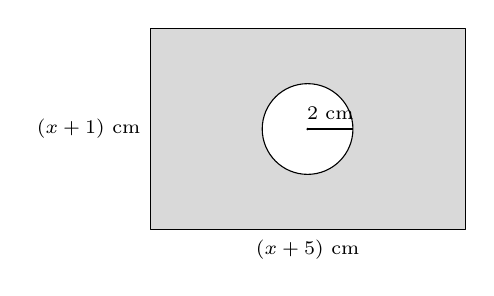
\begin{tikzpicture}[scale=0.8, font=\scriptsize, line join=round]
	\fill[gray!30] (0,0) rectangle (5,3.2);
	\fill[white] (2.5,1.6) circle (0.72);
	\draw (0,0) rectangle (5,3.2);
	\draw (2.5,1.6) circle (0.72);
	\draw (2.5,1.6)--(3.22,1.6);
	\node[above] at (2.86,1.6) {$2$ cm};
	\node[below] at (2.5,0) {$(x+5)$ cm};
	\node[left] at (0,1.6) {$(x+1)$ cm};
	\fill (2.5,1.6) circle (0.6pt);
\end{tikzpicture}
}
\loigiai{
\begin{enumerate}
\item Diện tích hình chữ nhật là
\[
S_{\text{cn}}=(x+5)(x+1)=x^2+6x+5\ \text{(cm}^2\text{)}.
\]
Diện tích hình tròn bán kính $2$ cm là
\[
S_{\text{tròn}}=\pi\cdot 2^2=4\pi\ \text{(cm}^2\text{)}.
\]
Diện tích phần tô đậm là
\[
S=S_{\text{cn}}-S_{\text{tròn}}=x^2+6x+5-4\pi\ \text{(cm}^2\text{)}.
\]

\item Ta có
\begin{align*}
x^2+6x+5-4\pi&=32-4\pi\\
x^2+6x+5&=32\\
x^2+6x-27&=0\\
(x+9)(x-3)&=0.
\end{align*}
Suy ra $x=-9$ hoặc $x=3$.

Vì $x>0$ nên $x=-9$ bị loại. Với $x=3$, hình chữ nhật có chiều dài $8$ cm và chiều rộng $4$ cm. Đường kính hình tròn bằng $4$ cm nên hình tròn tiếp xúc hai cạnh chiều rộng và nằm trọn trong hình chữ nhật.

Vậy $x=3$ cm.
\end{enumerate}
}
\end{bt}

%Bài 5
\begin{bt}[1,0 điểm]
\immini[thm]
{Một đường chạy bộ là hình vành khuyên tâm $O$. Bán kính mép trong là $5$ m và diện tích mặt đường chạy là $75\pi$ (m$^2$). Hai bán kính $OA$, $OB$ của mép ngoài tạo góc $\widehat{AOB}=60^\circ$ (hình vẽ).
\begin{enumerate}
\item Tính bán kính mép ngoài của đường chạy.
\item Tính độ dài cung nhỏ $AB$ và diện tích phần đường chạy nằm trong góc $\widehat{AOB}$.
\end{enumerate}
}
{
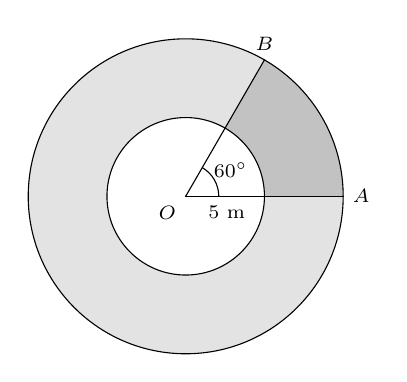
\begin{tikzpicture}[scale=0.2, font=\scriptsize, line join=round]
	\fill[gray!22] (0,0) circle (10);
	\fill[white] (0,0) circle (5);
	\fill[gray!48] (5,0) arc (0:60:5) -- (60:10) arc (60:0:10) -- cycle;
	\draw (0,0) circle (5);
	\draw (0,0) circle (10);
	\draw (0,0)--(10,0);
	\draw (0,0)--(60:10);
	\draw (2.1,0) arc (0:60:2.1);
	\node at (30:3.3) {$60^\circ$};
	\node[below] at (2.6,0) {$5$ m};
	\fill (0,0) circle (1.4pt) node[below left] {$O$};
	\fill (10,0) circle (1.4pt) node[right] {$A$};
	\fill (60:10) circle (1.4pt) node[above] {$B$};
\end{tikzpicture}
}
\loigiai{
\begin{enumerate}
\item Gọi $R$ (m) là bán kính mép ngoài, $R>5$. Diện tích hình vành khuyên là
\begin{align*}
\pi R^2-\pi\cdot 5^2&=75\pi\\
R^2-25&=75\\
R^2&=100.
\end{align*}
Vì $R>0$ nên $R=10$.

Vậy bán kính mép ngoài là $10$ m.

\item Cung nhỏ $AB$ thuộc đường tròn bán kính $10$ m và chắn góc ở tâm $60^\circ$, nên
\[
\ell_{\overset{\frown}{AB}}
=\dfrac{\pi Rn}{180}
=\dfrac{\pi\cdot 10\cdot 60}{180}
=\dfrac{10\pi}{3}\ \text{(m)}.
\]
Phần đường chạy trong góc $\widehat{AOB}$ là hình quạt vành khuyên, bằng hiệu hai hình quạt cùng góc $60^\circ$:
\begin{align*}
S
&=\dfrac{60}{360}\pi\cdot 10^2-\dfrac{60}{360}\pi\cdot 5^2\\
&=\dfrac{1}{6}\pi(100-25)\\
&=\dfrac{75\pi}{6}
=\dfrac{25\pi}{2}\ \text{(m}^2\text{)}.
\end{align*}
Vậy cung nhỏ $AB$ dài $\dfrac{10\pi}{3}$ m và phần đường chạy trong góc $\widehat{AOB}$ có diện tích $\dfrac{25\pi}{2}$ m$^2$.
\end{enumerate}
}
\end{bt}

%Câu 6

\begin{bt}
	Cho nửa đường tròn $(O;R)$ có đường kính $MN$. Kẻ hai tiếp tuyến $Mx$ và $Ny$ của nửa đường tròn $(O)$ ($Mx$, $Ny$ và nửa đường tròn $(O)$ thuộc cùng một phía của đường thẳng $MN$). Lấy điểm $A$ bất kỳ thuộc nửa đường tròn $(O)$ ($AM<AN$). Qua $A$, kẻ tiếp tuyến với nửa đường tròn $(O)$ cắt $Mx$ và $Ny$ lần lượt tại $E$ và $F$.
	
	\begin{listEX}[1]
	\item Chứng minh $4$ điểm $M,E,A,O$ cùng thuộc một đường tròn.
	\item Chứng minh $ME+NF=EF$ và $AE\cdot AF=R^2$.
	\item Gọi $H$ là giao điểm của $MF$ và $NE$, $AH$ cắt $MN$ tại $K$. Chứng minh $AK\perp MN$ và $H$ là trung điểm của $AK$.
	\end{listEX}
\end{bt}
\Closesolutionfile{ansbook}
